% !TEX root =../LibroTipoETSI.tex
\chapter{Ejemplo de Capítulo de Problemas}\LABCHAP{CAPPB}

\epigraph{Este es un ejemplo de capítulo de libro de problemas, donde cada sección es un problema distinto, con 
enunciado y solución. Se incluye un problema cualquiera, para que el lector pueda aprender cómo utilizarlo. El enunciado de cada problema comienza con \comando{problema} cómo si se tratara de una sección más. Como tal aparecerá en el índice del libro y en las cabeceras de páginas correspondientes.} 

\lettrine[lraise=-0.1, lines=2, loversize=0.25]{B}{la} bla,..., los conceptos más relevantes necesarios para la resolución de los problemas de este capítulo se refiere al lector al texto \cite{Hernando08}. La notación es la incluida al comienzo de este documento.
%
%incluyeron en los Apartados \SSEC{Ruido}, \SSEC{Sensibilidad}, y \SSEC{Nolinealidad}. 
Los conceptos necesarios para resolver los problemas planteados se pueden consultar en \cite{Murillo07}, excepto los relacionados con el cálculo de propagación, para los que se puede recurrir a \cite{Hernando08}. A continuación se incluye una descripción de los cálculos más relevantes utilizados en estos problemas, utilizando la notación introducida al comienzo del texto.


\section{Ruido y sensibilidad}\LABSEC{Ruido}
Vamos a estudiar el ruido y la sensibilidad en ...

\subsection{Temperatura y figura de ruido} \LABSSEC{Ruido}
En este texto, ver comienzo del mismo, se denota por $f_r$ y $T_r$ la figura y la temperatura equivalente de ruido, respectivamente, del receptor, formado éste por los elementos que van desde el conector de antena a la entrada al demodulador. Por otro lado, $f_a$ y $T_a$ se utilizan para denotar la figura y la temperatura equivalente de ruido de la antena. Y $f_s$ y $T_s$ denotan la figura de ruido y la temperatura equivalente del sistema completo, antena más receptor.  Aquí las figuras de ruido están en unidades naturales, y las denotamos por ello en minúsculas. La misma notación para las figuras de ruido en mayúsculas se utilizará para denotar dB. (...)%Por otra parte, se asume adaptación de impedancias en el sistema. 


\subsection{Sensibilidad}\LABSSEC{Sensibilidad}


En radiocomunicaciones digitales es habitual utilizar \cite{Hernando08}
\begin{align}
    \frac{c}{n}=\frac{e_b/T_b}{n_0\cdot B}=\frac{e_b\cdot R_b}{n_0\cdot B},
\end{align}
donde $c$ es la potencia de portadora en u.n., $B$ es el ancho de banda equivalente de ruido y
%\begin{align}
%    w&=\frac{c}{n}\cdot \frac{B}{R_b},
%\end{align}
%donde
$R_b=1/T_b$ es el régimen binario. 
%En comunicaciones digitales, si se utiliza el filtro adaptado como filtro receptor, $B=1/T_s$, y $\frac{c}{n}=\log_2M\cdot w$.

Por otro lado se define $w=e_b/n_0$ como (...)

\section{No linealidad}\LABSSEC{Nolinealidad}
Si la sensibilidad nos impone un mínimo a la potencia mínima recibida, el cálculo de la distorsión por no linealidad permite determinar la potencia máxima que el receptor, o transmisor, puede manejar. 
La distorsión por no linealidad de un dispositivo se mide de diferentes formas. Una de las más utilizadas es calcular la relación esperada entre la potencia útil a la salida, $P_o$, y la potencia de intermodulación de tercer orden, $I_3$. Esta relación, una diferencia si se escribe en decibelios, se denota por relación de protección frente a intermodulación de tercer orden, $RP=P_o-I_3$.

Para calcular este valor se (...)


\problema[Radioenlace del servicio fijo a 13 GHz]{Radioenlace del servicio fijo a 13 GHz. Título muy largo que en realidad no cabría en la cabecera}

Una compañía de telefonía móvil desea instalar un radioenlace digital del servicio fijo a $13$ GHz, para unir dos estaciones base a través de un vano de $15$ km de longitud. El enlace tiene un obstáculo agudo de incidencia rasante, esto es, con despejamiento $h=0$ y que introduce unas pérdidas de 6 dB a la par que evita cualquier reflexión en el suelo. 

Se propone utilizar para ello equipos de la serie Flexi-Hopper de Nokia, cuyos datos se incluyen en la \TAB{resfFHop13} para una transmisión dúplex\footnote{ el $2\times$ indica que se utilizan las dos polarizaciones para transmitir.} de $2 \times 2$E1, resultando $4.2$ Mbps en cada sentido modulados en un radiocanal. Tanto el transmisor como el receptor constan de una unidad interior (IU), al pié de la torre, y una unidad exterior (OU) con la etapa de RF junto a la antena, en el extremo superior de las torres, de 15 m. Se sabe, además, que hay una probabilidad $\eta = 25.73$ \% de que exista actividad multitrayecto en el vano para esa zona climática. Además, para esa zona climática se conoce la atenuación, $A_p$, excedida en el $p$\% del tiempo, ver \FIG{resfFHop13}. 

El operador ha fijado como criterios de calidad el \% del tiempo en el que el sistema sufre interrupciones largas y cortas, y como objetivos que las primeras ($>10$s, $BER>10^{-3}$) no superen el $0.036\%$ y las cortas ($\leq10$s, $BER>10^{-3}$) no superen el 0.006\% anual. El departamento de radio tiene que calcular la mínima potencia transmitida para la que el enlace es viable, evitando así interferencias a otros sistemas. 
 
Se pide 
\begin{enumerate}%[labelindent=\parindent,leftmargin=\parindent, label=\normalfont\bfseries  \alph*)] 
\item Calcular el valor de esta potencia. Indique si es necesario mantener en el diseño el HSB (Hot Stand By).
\end{enumerate}   

\begin{table}[h]
%\small
\caption{Datos de las estaciones, con equipos Flexi-Hopper de Nokia}
\begin{center}
\begin{tabular}{p{8.5cm}p{2.5cm}}
 \hline
Potencia transmitida	(entregada a antena) regulable & -5 a 20 dBm	\\
Ganancia antenas & $40.5$ dBi\\	
Modulación & $\pi/4$-DQPSK\\
%Pérdidas en conectores 1 dB	\\
Potencia recibida necesaria para  $BER = 10^{-3}$ y 2E1 ($4.2$Mbps) & $P_{dr}=-89$ dBm\\
Figura de ruido del sistema & 6 dB\\
HSB 1+1, tanto en OU e IU &\\
Tiempo medio entre fallos para OU & $MTBF$=35 años \\
Tiempo medio entre fallos para IU $MTBF$=110 años \\
Tiempo medio en reparar para OU como IU & $MTTR$=20 horas\\
%Altura de antenas sobre el suelo, 15 m\\
Signatura normalizada del receptor	& $k = log_2 M$ \\
 $M$ el número de puntos de la constelación de la modulación & \\
 \hline
\end{tabular}
\end{center}
\LABTAB{resfFHop13}
\end{table}%
\begin{figure}[h]
\centering 
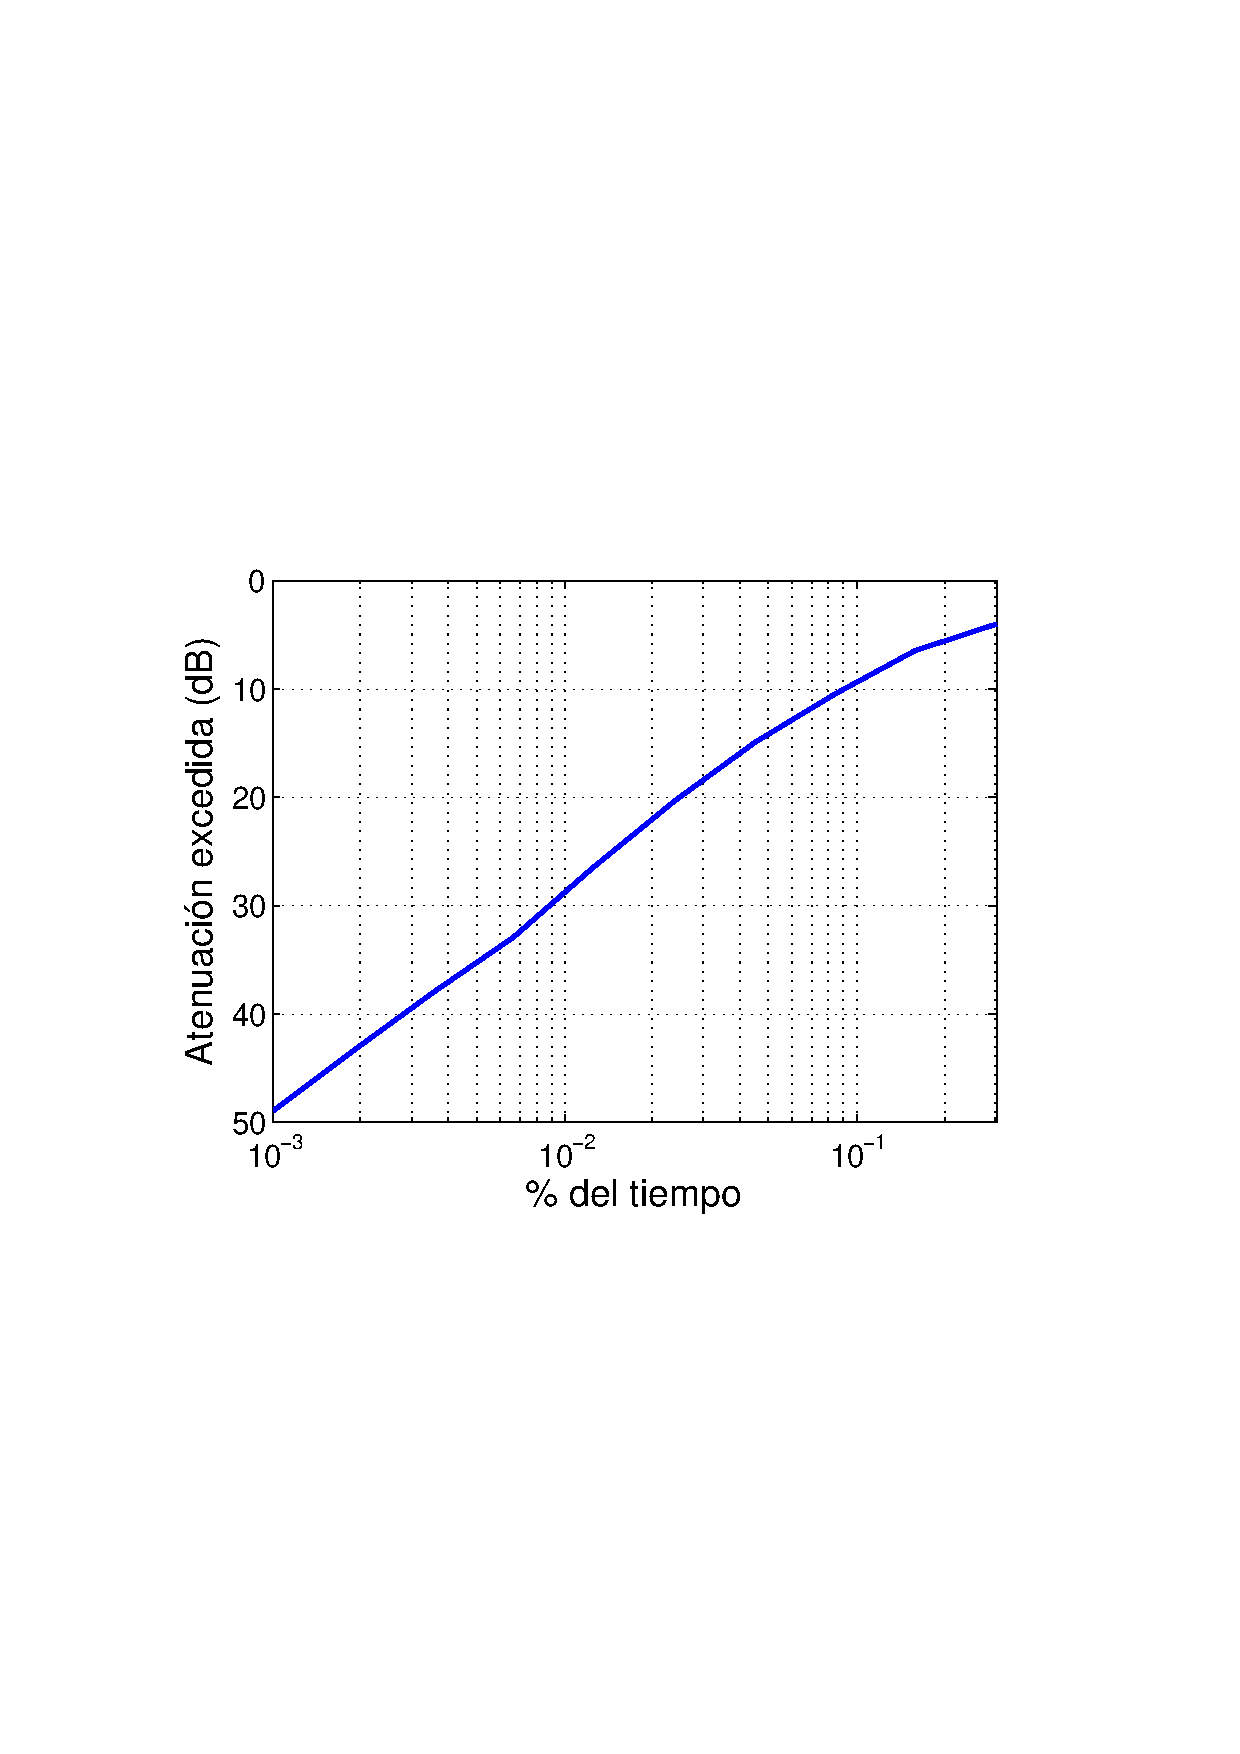
\includegraphics[width=8 cm]{CapituloProblemasLibroETSI/figuras/rain13GHz.pdf}
\caption{Atenuación por lluvia excedida en el $p$ \% del tiempo para 13 GHz y 15 km de distancia}\LABFIG{resfFHop13}%\vspace{-.5 cm}
\end{figure} 

 \begin{solnum}
 \item 
En principio la frecuencia de trabajo no es muy alta, lo que hace pensar que el enlace no estará limitado por lluvia. Los tiempos medios entre fallos son grandes, lo que parece indicar que la indisponibilidad, o interruciones largas, no va a ser un problema. Mientras que sí lo será la pérdida de fidelidad, o interrupciones breves. En todo caso, como el régimen binario es bajo, $\leq 34$ Mbps, el desvanecimiento selectivo no es importante. 

El margen bruto es el que domina en ambos criterios de calidad. De forma que podemos calcular el margen necesario para que se cumplan los objetivos de interrupciones largas (indisponibilidad) y cortas (fidelidad) y quedarnos con el más restrictivo, el mayor.

Calculamos primero el margen necesario para que se cumpla la indisponibilidad. La indisponibilidad de equipos sería la resultante de la suma de la indiponibilidad en cada extremo. En cada extremo tenemos dos equipos funcionando, la IU y la OU, el $MTBF$ equivalente es
\begin{align}
MTBF_e&=(MTBF_{IU}^{-1}+MTFB_{OU}^{-1})^{-1}\nonumber\\
    &=((110\cdot24\cdot 365)^{-1}+(35\cdot24\cdot365)^{-1})^{-1}=2.3259\cdot 10^5.
\end{align}
 Y calculamos
\begin{align}
q&=MTTR/(MTTR+MTBF_e)=20/(20+2.3259\cdot 10^5)=8.5980\cdot 10^{-5}.
\end{align}
 para finalmente estimar la indisponibilidad
\begin{align}
U_{e}&=2 \cdot 100\cdot \binom{M+N}{N+1} (mq)^{N+1}\nonumber\\&=2\cdot 100 \cdot\binom{1+1}{1+1} (1\cdot 8.5980\cdot 10^{-5})^{1+1}
=1.478510^{-6}\%,
\end{align}
%Si no se tuviese HSB, tendríamos 
donde $m=1$ porque tenemos un vano y  $M=N=1$ porque el HSB (Hot Stand By) es $M+N=1+1$. Dado que el máximo valor permitido es $0.036\%$ y que el valor anterior de indisponibilidad por equipos es muy muy pequeño, el máximo valor permitido para indisponibilidad por propagación es, aproximadamente este mismo valor (...)\end{solnum}



%%%%%%%%%%%%
%%%%%%%%%%%%
%%%%%%%%%%%%

\problema{Radioenlace del servicio fijo a 13 GHz}

Una compañía de telefonía móvil desea instalar un radioenlace digital del servicio fijo a $13$ GHz, para unir dos estaciones base a través de un vano de $15$ km de longitud. El enlace tiene un obstáculo agudo de incidencia rasante, esto es, con despejamiento $h=0$ y que introduce unas pérdidas de 6 dB a la par que evita cualquier reflexión en el suelo. 

Se propone utilizar para ello equipos de la serie Flexi-Hopper de Nokia, cuyos datos se incluyen en la \TAB{resfFHop13} para una transmisión dúplex\footnote{ el $2\times$ indica que se utilizan las dos polarizaciones para transmitir.} de $2 \times 2$E1, resultando $4.2$ Mbps en cada sentido modulados en un radiocanal. Tanto el transmisor como el receptor constan de una unidad interior (IU), al pié de la torre, y una unidad exterior (OU) con la etapa de RF junto a la antena, en el extremo superior de las torres, de 15 m. Se sabe, además, que hay una probabilidad $\eta = 25.73$ \% de que exista actividad multitrayecto en el vano para esa zona climática. Además, para esa zona climática se conoce la atenuación, $A_p$, excedida en el $p$\% del tiempo, ver \FIG{resfFHop13}. 

El operador ha fijado como criterios de calidad el \% del tiempo en el que el sistema sufre interrupciones largas y cortas, y como objetivos que las primeras ($>10$s, $BER>10^{-3}$) no superen el $0.036\%$ y las cortas ($\leq10$s, $BER>10^{-3}$) no superen el 0.006\% anual. El departamento de radio tiene que calcular la mínima potencia transmitida para la que el enlace es viable, evitando así interferencias a otros sistemas. 
 
Se pide 
\begin{enumerate}%[labelindent=\parindent,leftmargin=\parindent, label=\normalfont\bfseries  \alph*)] 
\item Calcular el valor de esta potencia. Indique si es necesario mantener en el diseño el HSB (Hot Stand By).
\end{enumerate}   

\begin{table}[h]
%\small
\caption{Datos de las estaciones, con equipos Flexi-Hopper de Nokia}
\begin{center}
\begin{tabular}{p{8.5cm}p{2.5cm}}
 \hline
Potencia transmitida	(entregada a antena) regulable & -5 a 20 dBm	\\
Ganancia antenas & $40.5$ dBi\\	
Modulación & $\pi/4$-DQPSK\\
%Pérdidas en conectores 1 dB	\\
Potencia recibida necesaria para  $BER = 10^{-3}$ y 2E1 ($4.2$Mbps) & $P_{dr}=-89$ dBm\\
Figura de ruido del sistema & 6 dB\\
HSB 1+1, tanto en OU e IU &\\
Tiempo medio entre fallos para OU & $MTBF$=35 años \\
Tiempo medio entre fallos para IU $MTBF$=110 años \\
Tiempo medio en reparar para OU como IU & $MTTR$=20 horas\\
%Altura de antenas sobre el suelo, 15 m\\
Signatura normalizada del receptor	& $k = log_2 M$ \\
 $M$ el número de puntos de la constelación de la modulación & \\
 \hline
\end{tabular}
\end{center}
\LABTAB{resfFHop13}
\end{table}%
\begin{figure}[h]
\centering 
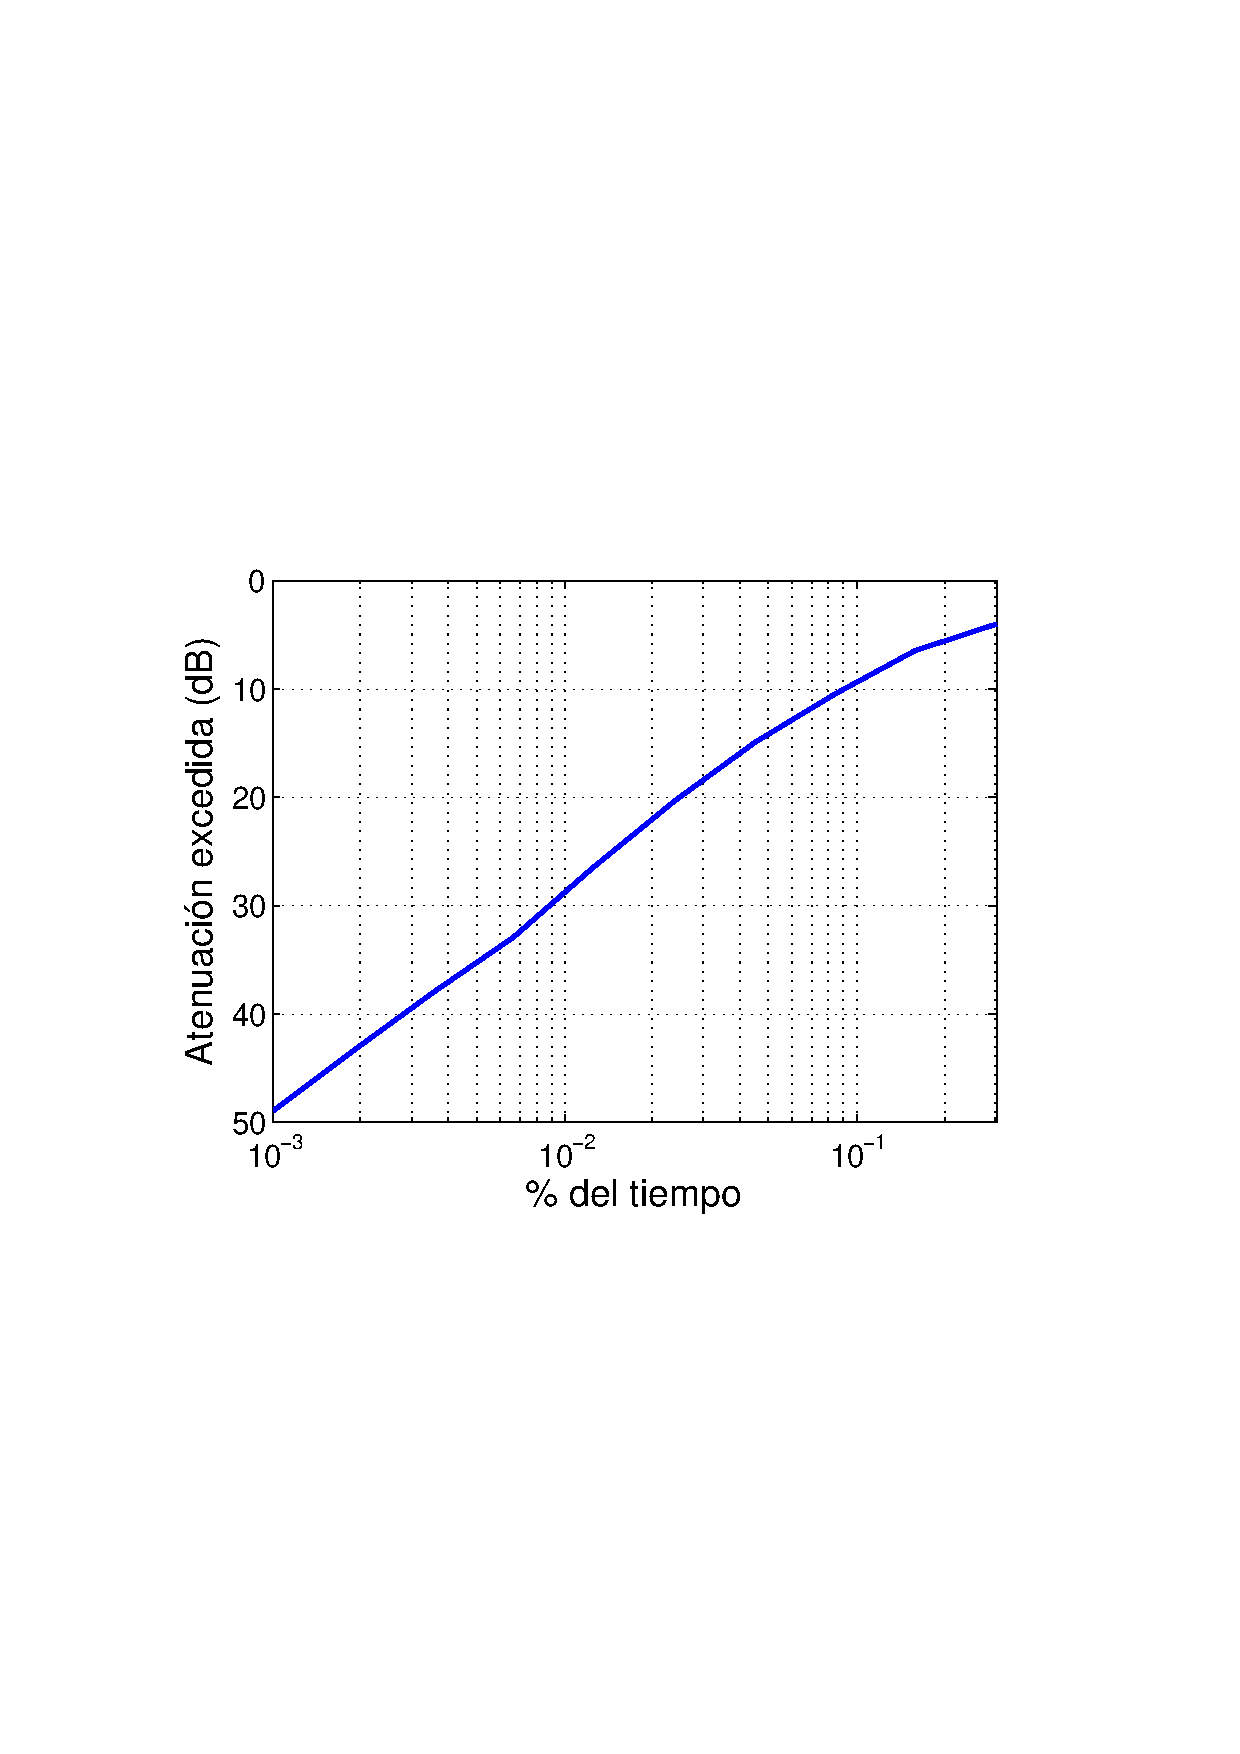
\includegraphics[width=8 cm]{CapituloProblemasLibroETSI/figuras/rain13GHz.pdf}
\caption{Atenuación por lluvia excedida en el $p$ \% del tiempo para 13 GHz y 15 km de distancia}\LABFIG{resfFHop13}%\vspace{-.5 cm}
\end{figure} 

%%%%%%%%%%%
%%%%%%%%%%%
%%%%%%%%%%%

\section{...Ruido y sensibilidad}\LABSEC{Ruido}
Vamos a estudiar el ruido y la sensibilidad en ...

\subsection{...Temperatura y figura de ruido} \LABSSEC{Ruido}
En este texto, ver comienzo del mismo, se denota por $f_r$ y $T_r$ la figura y la temperatura equivalente de ruido, respectivamente, del receptor, formado éste por los elementos que van desde el conector de antena a la entrada al demodulador. Por otro lado, $f_a$ y $T_a$ se utilizan para denotar la figura y la temperatura equivalente de ruido de la antena. Y $f_s$ y $T_s$ denotan la figura de ruido y la temperatura equivalente del sistema completo, antena más receptor.  Aquí las figuras de ruido están en unidades naturales, y las denotamos por ello en minúsculas. La misma notación para las figuras de ruido en mayúsculas se utilizará para denotar dB. (...)%Por otra parte, se asume adaptación de impedancias en el sistema. 

\subsection{...Temperatura y figura de ruido} \LABSSEC{Ruido}
... En este texto, ver comienzo del mismo, se denota por $f_r$ y $T_r$ la figura y la temperatura equivalente de ruido, respectivamente, del receptor, formado éste por los elementos que van desde el conector de antena a la entrada al demodulador. Por otro lado, $f_a$ y $T_a$ se utilizan para denotar la figura y la temperatura equivalente de ruido de la antena. Y $f_s$ y $T_s$ denotan la figura de ruido y la temperatura equivalente del sistema completo, antena más receptor.  Aquí las figuras de ruido están en unidades naturales, y las denotamos por ello en minúsculas. La misma notación para las figuras de ruido en mayúsculas se utilizará para denotar dB. (...)%Por otra parte, se asume adaptación de impedancias en el sistema. 

\subsection{...Temperatura y figura de ruido} \LABSSEC{Ruido}
... En este texto, ver comienzo del mismo, se denota por $f_r$ y $T_r$ la figura y la temperatura equivalente de ruido, respectivamente, del receptor, formado éste por los elementos que van desde el conector de antena a la entrada al demodulador. Por otro lado, $f_a$ y $T_a$ se utilizan para denotar la figura y la temperatura equivalente de ruido de la antena. Y $f_s$ y $T_s$ denotan la figura de ruido y la temperatura equivalente del sistema completo, antena más receptor.  Aquí las figuras de ruido están en unidades naturales, y las denotamos por ello en minúsculas. La misma notación para las figuras de ruido en mayúsculas se utilizará para denotar dB. (...)%Por otra parte, se asume adaptación de impedancias en el sistema. 

%Para incluir otro problema, utilice \problema
\endinput
